\documentclass{article}
\usepackage[a4paper,left=3cm,right=3cm,top=3cm,bottom=3cm]{geometry}
\usepackage[utf8]{inputenc}
\usepackage[T1]{fontenc}
\usepackage{latexsym,amsfonts,amsmath,amssymb,amstext,graphicx,titlesec,ae,aecompl,mathtools,tabularx, multirow, cancel, nicefrac,subcaption, blindtext, floatrow}
\setlength{\parindent}{0pt}
\newfloatcommand{capbtabbox}{table}[][\FBwidth]


\begin{document}

\begin{titlepage}
       \begin{center}
             \begin{huge}
				   %% Update assignment number here
                   \textbf{Assignment 2}
             \end{huge}
       \end{center}

       \begin{center}
             \begin{large}
                   Computational Intelligence, SS2020
             \end{large}
       \end{center}

       \begin{center}
 \begin{tabularx}{\textwidth}{|>{\hsize=.33\hsize}X|>{\hsize=.33\hsize}X|>{\hsize=.33\hsize}X|} 

                   \hline
                   \multicolumn{3}{|c|}{\textbf{Team Members}} \\
                   \hline
                   Last name & First name & Matriculation Number \\
                   \hline
                   Blöcher & Christian & 01573246 \\
                   \hline
                   Bürgener & Max & 01531577 \\
                   \hline
                    &  &  \\
                   \hline

             \end{tabularx}
       \end{center}
\end{titlepage}

\section{Linear regression}

\subsection{Derivation of Regularized Linear Regression}

\begin{itemize}
    
    \item Why is the design matrix $\boldsymbol{X}$ containing $n + 1$ and not just $n$?
    
    \begin{itemize} 
    
        \item The simplest form of linear regression is calculated by:
            $$\boldsymbol{y}(\boldsymbol{x, \omega}) = \underset{bias}{\underbrace{\boldsymbol{\omega_0}}} + \boldsymbol{X} \boldsymbol{\omega}$$
        \item Modifying $\boldsymbol{X}$ with the additional column. The addition of the bias $\omega_0$ is compensated and the calculation simplified. \\
      
            $$ \boldsymbol{y} = 
            \begin{bmatrix}
	            1		& \dots		& x_1	\\
	            \vdots	& \ddots 	& \vdots		\\
	            1		& \dots 		& x_N
	            \end{bmatrix}
	            \begin{bmatrix}
	            \omega_0 \\
	            \vdots	 \\
	            \omega_N	 
            \end{bmatrix} $$
     \end{itemize}
    
    \item What is the dimension of the gradient vector?
    
    \begin{itemize}
        \item The gradient contains the derivation of all $J\boldsymbol{(\theta)}$ for all variables. That means the gradient has the dimension $m \times 1$ and it contains a group of targets. \\        
            $$\frac{\partial J(\boldsymbol{\boldsymbol{\theta)}}}{\partial \boldsymbol{\theta}} =
            \begin{bmatrix}
            	\frac{\partial J(\boldsymbol{\theta)}}{\partial \theta_1}	 \\
            	\vdots \\
            	\frac{\partial J(\boldsymbol{\theta)}}{\partial \theta_m}  	
            \end{bmatrix}$$     
    \end{itemize} 
    
    \item What is the definition of the Jacobian matrix and what is the difference between the gradient and the Jacobian matrix?
    
    \begin{itemize}
        \item The Jacobian matrix elements are calculated by the derivatives of all elements of a vector with respect to all variables.  \\
            $$ \boldsymbol{J} = 
            \begin{bmatrix}
            	\frac{\partial y_1}{\partial x_1}	&	\dots	&	\frac{\partial y_1}{\partial x_n} 	\\
            	\vdots								&	\ddots	&	\vdots								\\
            	\frac{\partial y_m}{\partial x_1	}	&	\dots	&	\frac{\partial y_m}{\partial x_n}
            \end{bmatrix} $$
            
        \item The gradient is computed from a scalar. It is a vector which contains the derivatives of a function for all variables.              
    \end{itemize}
    
    \item What is the dimension of the Jacobian matrix and what is it equal to?
    
    \begin{itemize}
    
        \item The dimension of the Jacobian matrix not only equal the dimension of the Design matrix, but the result itself is the Design matrix. Because $\frac{\partial\boldsymbol{Ab}}{\partial\boldsymbol{b}}=\boldsymbol{A}$:
        
        $$ \boldsymbol{J} = \frac{\partial \boldsymbol{X\theta}}{\partial\boldsymbol{\theta}} = \boldsymbol{X}
$$    
    \end{itemize}
    
    \item Minimization of the regularized linear regression cost function
    
    $$\begin{array}{rclr}
        J(\boldsymbol{\theta}) & = & \frac{1}{m} \| \boldsymbol{X\theta - y} \|^2 + \frac{\lambda}{m} \| \boldsymbol{\theta}^2 \| & \\\\
        J(\boldsymbol{\theta}) & = & \frac{1}{m} \left[(\boldsymbol{X\theta - y})^T \cdot (\boldsymbol{X\theta - y}) \right] + \frac{\lambda}{m} (\boldsymbol{\theta^T \theta}) & \mid \frac{\partial}{\partial\boldsymbol{\theta}} \\
      \end{array}$$
    
      \textrm{Using Hint 2 from our exercise sheet the calculation is simplified to:} \\
    
    $$\begin{array}{rclr}
        \frac{\partial J(\boldsymbol{\theta})}{\partial \boldsymbol{\theta}} & = & \frac{2}{m}(\boldsymbol{X\theta - y})^T \cdot \boldsymbol{X} + \frac{2\lambda}{m}\ \boldsymbol{\theta}^T & 
    \end{array}$$

    We set the gradient to zero to calculate our solution $\theta$.	Due to the property of transpose: $ (\boldsymbol{A}\boldsymbol{B})^T = \boldsymbol{B}^T\boldsymbol{A}^T $ we get:
    
    $$\begin{array}{rclr}    
    \frac{2}{m}(\boldsymbol{\theta}^T \boldsymbol{X}^T \boldsymbol{X} - \boldsymbol{y}^T \boldsymbol{X}) + \frac{2\lambda}{m}\boldsymbol{\theta}^T & = & 0 \\\\
    \boldsymbol{\theta}^T \boldsymbol{X}^T \boldsymbol{X} + \lambda \boldsymbol{\theta}^T & = & \boldsymbol{y}^T \boldsymbol{X} & \\\\
    \boldsymbol{\theta}^T (\boldsymbol{X}^T \boldsymbol{X} + \lambda \boldsymbol{I}) & = & \boldsymbol{y}^T\boldsymbol{X} & \\\\
    \boldsymbol{\theta}^T & = & (\boldsymbol{y}^T \boldsymbol{X})(\boldsymbol{X}^T \boldsymbol{X} + \lambda \boldsymbol{I})^{-1} & \mid ()^T \\\\
    \end{array}$$

	
	$$\begin{array}{rcl}
	
    \theta & = & (\boldsymbol{X}^T\boldsymbol{X} + \lambda\boldsymbol{I})^{-1^T} (\boldsymbol{y}^T\boldsymbol{X})^T \\\\
    \theta & = & (\boldsymbol{X}^T\boldsymbol{X} + \lambda\boldsymbol{I})^{-1} (\boldsymbol{X}^T\boldsymbol{y})
	\end{array}$$
    
\end{itemize}

\newpage

\subsection{Linear Regression with polynomial features}


\begin{figure}[!ht]
\centering
\makebox[\textwidth]{
\begin{subfigure}{0.65\textwidth}
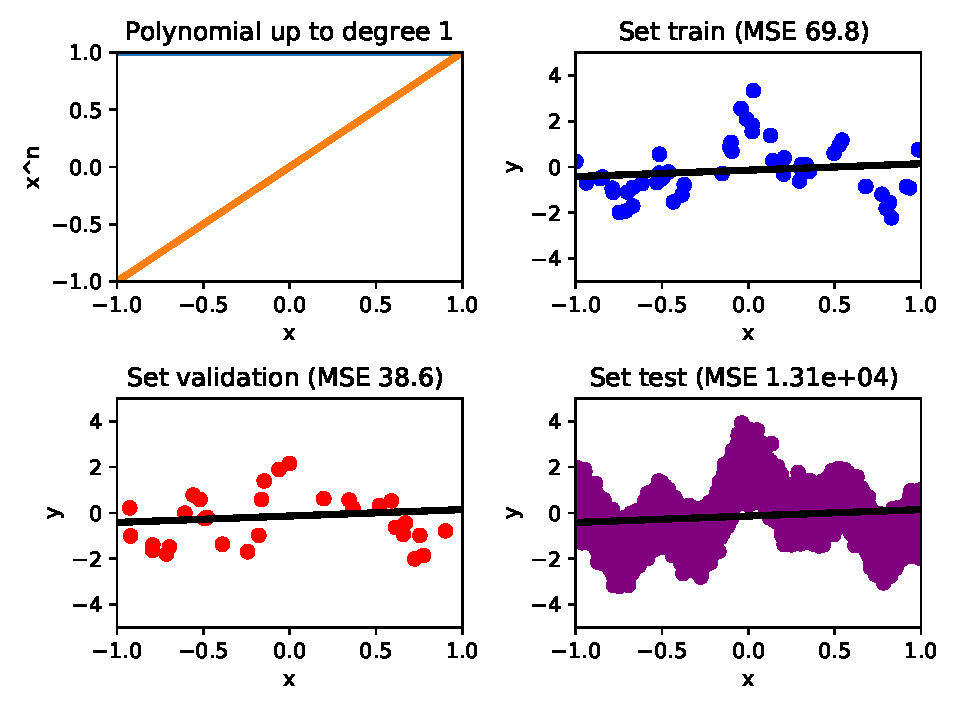
\includegraphics[width=\textwidth]{./Figures/linreg_poly1_deg1.pdf}
\caption{$n=1$}
\end{subfigure}
\begin{subfigure}{0.65\textwidth}
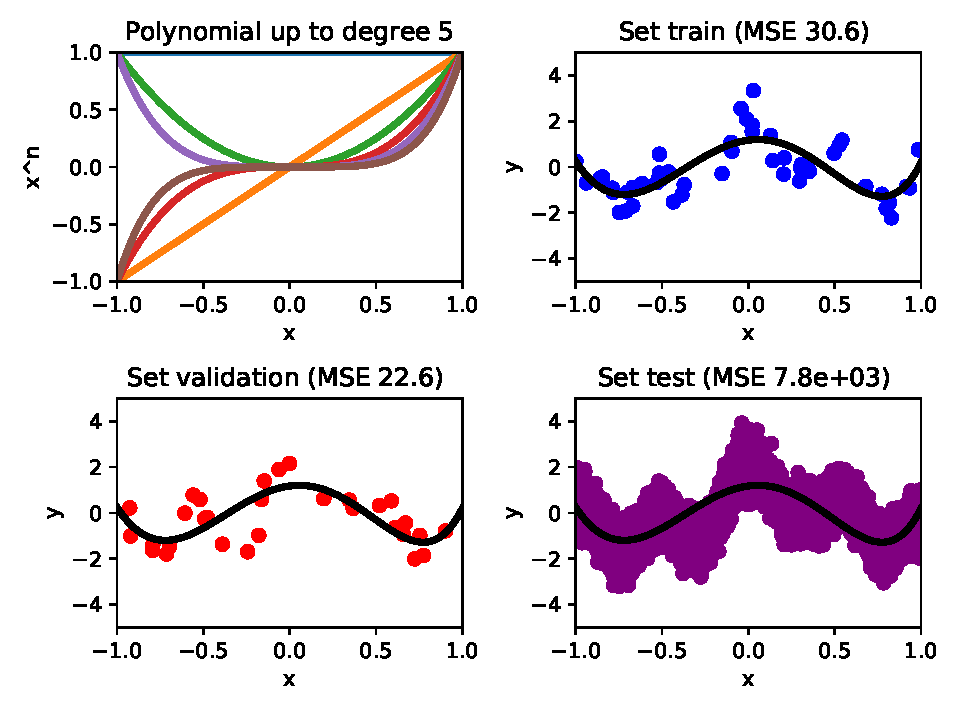
\includegraphics[width=\textwidth]{./Figures/linreg_poly1_deg5.pdf}
\caption{$n=5$}
\end{subfigure}
}

\makebox[\textwidth]{
\begin{subfigure}{0.65\textwidth}
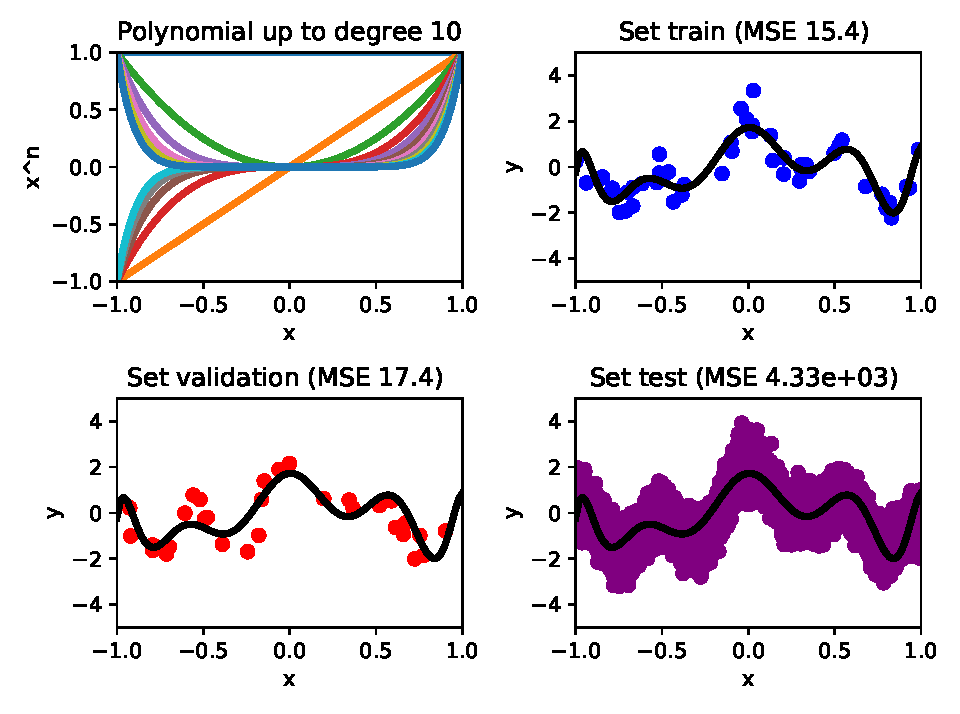
\includegraphics[width=\textwidth]{./Figures/linreg_poly1_deg10.pdf}
\caption{$n=10$}
\end{subfigure}
\begin{subfigure}{0.65\textwidth}
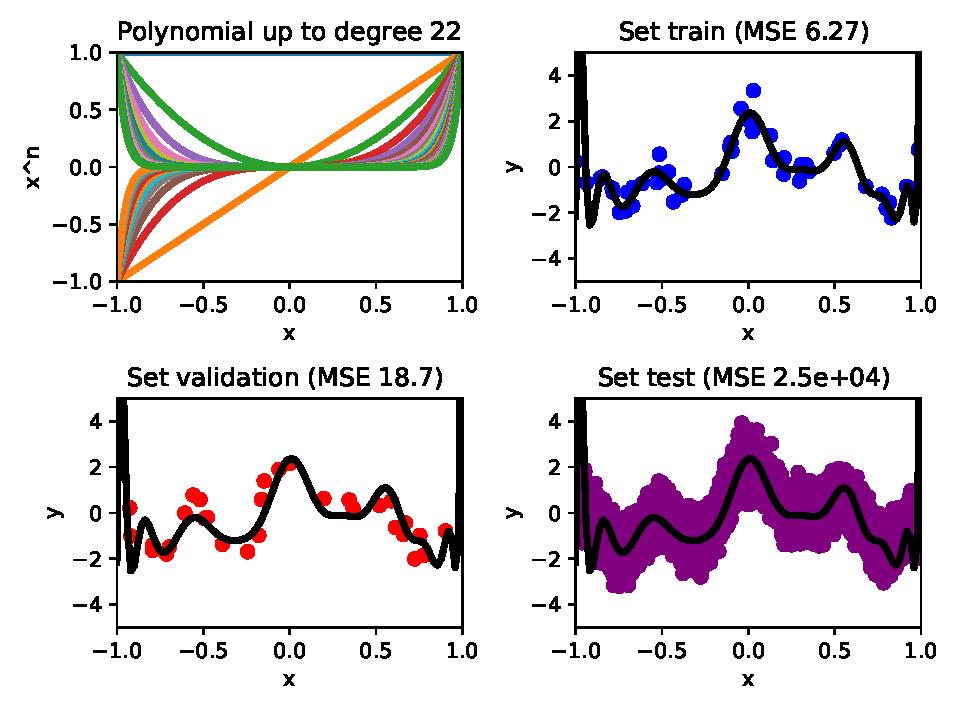
\includegraphics[width=\textwidth]{./Figures/linreg_poly1_deg22.pdf}
\caption{$n=22$}
\end{subfigure}
}
\caption{Results of Linear Regression for varying polynomial degree $n$.}
\label{linreg_poly1}
\end{figure}

\begin{figure}[!ht]
\makebox[\textwidth]{
\begin{subfigure}{0.65\textwidth}
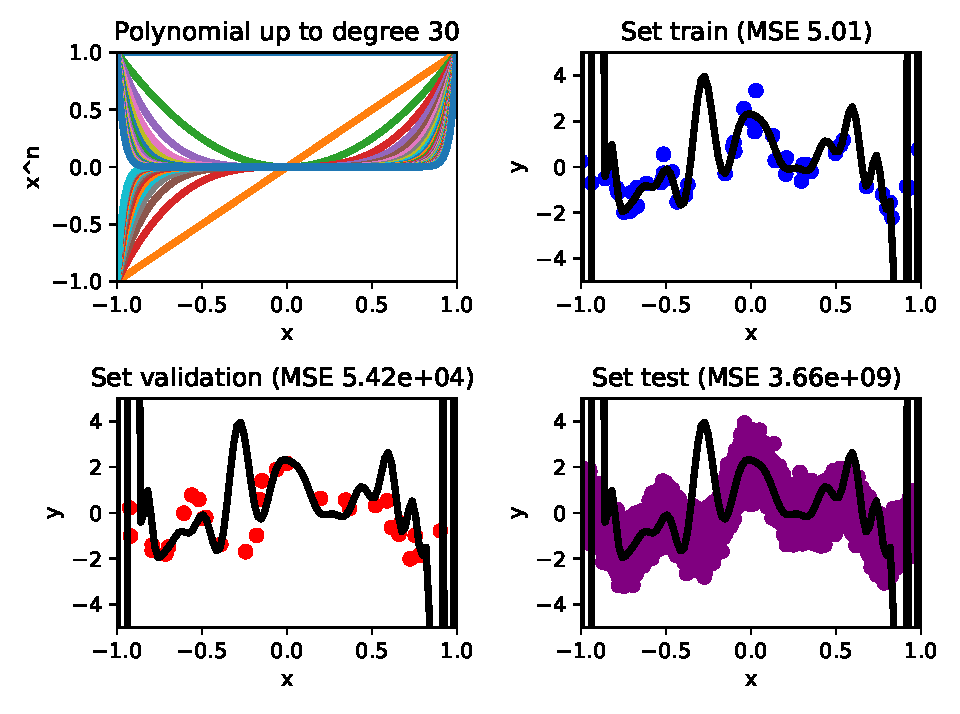
\includegraphics[width=\textwidth]{./Figures/linreg_poly2_besttrain.pdf}
\caption{Training set, $n=30$}
\end{subfigure}
\begin{subfigure}{0.65\textwidth}
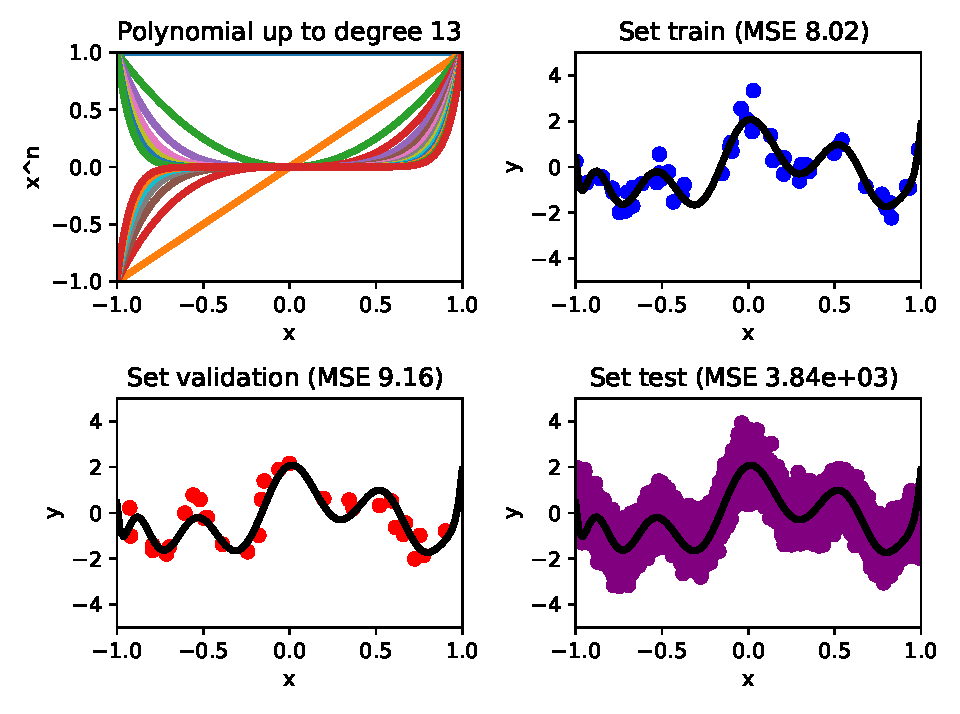
\includegraphics[width=\textwidth]{./Figures/linreg_poly3_bestval.pdf}
\caption{Validation set, $n=13$}
\end{subfigure}
}
\caption{Results with lowest cost on training and validation set.}
\label{linreg_poly23}
\end{figure}

\begin{figure}[!ht]
\centering
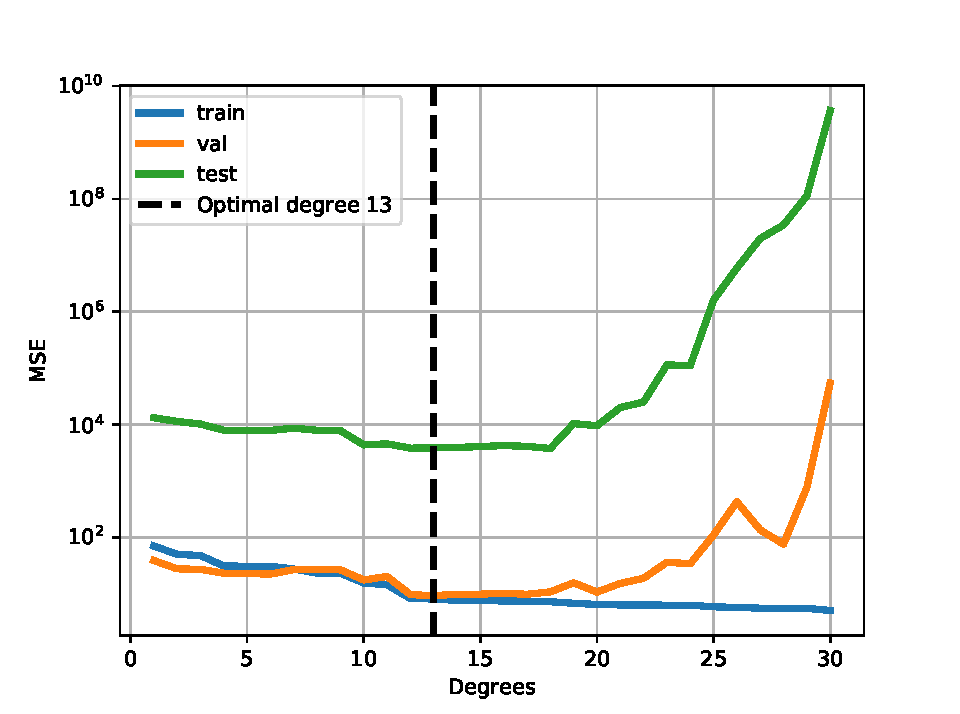
\includegraphics[width=0.8\textwidth]{./Figures/linreg_poly4_errors.pdf}
\caption{Training, validation and testing costs as a function of the polynomial degree $n$.}
\label{linreg_poly4}
\end{figure}

As can be seen in figure \ref{linreg_poly4} the training cost decreases with increasing polynomial degree $n$. That means the lowest cost on the training set can be achieved by using polynomials up to the highest degree $n=30$ (s. figure \ref{linreg_poly23}), but then the testing cost is maximised. This is due to overfitting: By finding parameters that suit the training data best, the solution becomes too specific for the validation and testing sets, leading to greater errors. Looking at figure \ref{linreg_poly23} all training data points are in the close vicinity of the polynomial but the output function barely resembles the data. The best results can be obtained with degree $n=13$, which minimises the validation cost (s. figure \ref{linreg_poly4}) and leads to a very low testing cost. Having a validation set in addition to the training set helps in finding the right degree for the linear regression process and greatly improves the quality of the solution.

\newpage


\subsection{(Bonus) Linear Regression with radial basis functions}

\begin{figure}[!ht]
\centering
\makebox[\textwidth]{
\begin{subfigure}{0.65\textwidth}
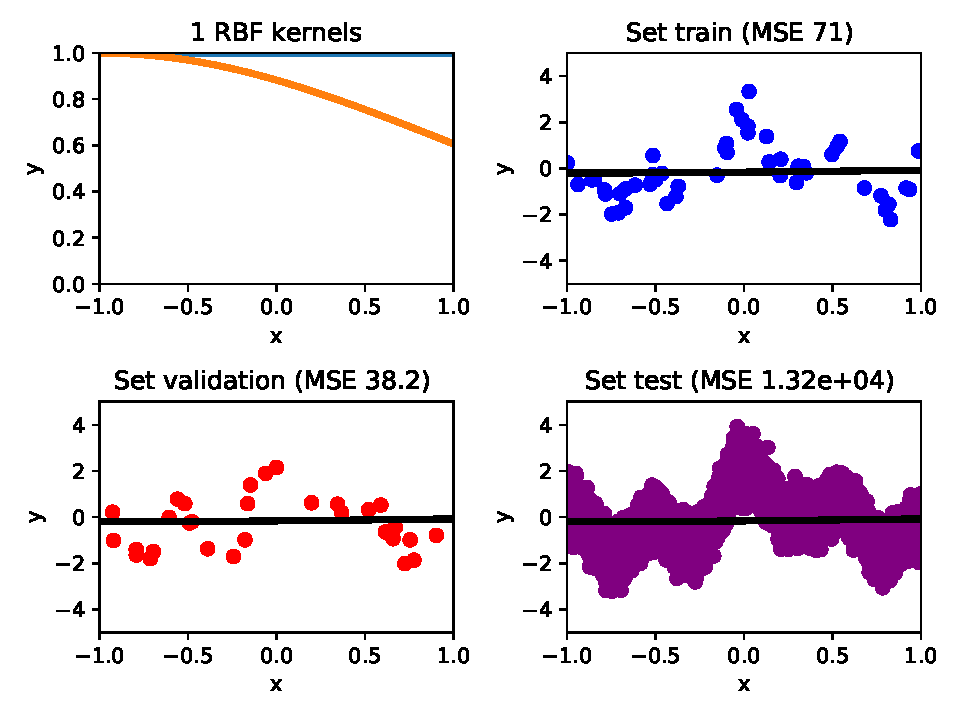
\includegraphics[width=\textwidth]{./Figures/linreg_rbf1_ncent1.pdf}
\caption{$l=1$}
\end{subfigure}
\begin{subfigure}{0.65\textwidth}
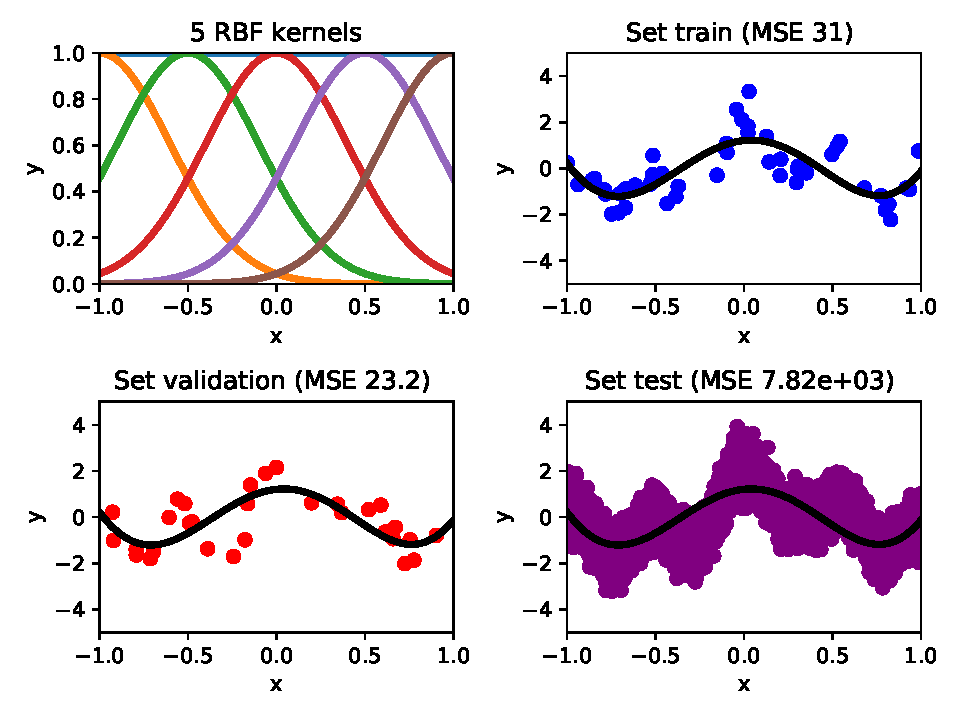
\includegraphics[width=\textwidth]{./Figures/linreg_rbf1_ncent5.pdf}
\caption{$l=5$}
\end{subfigure}
}

\makebox[\textwidth]{
\begin{subfigure}{0.65\textwidth}
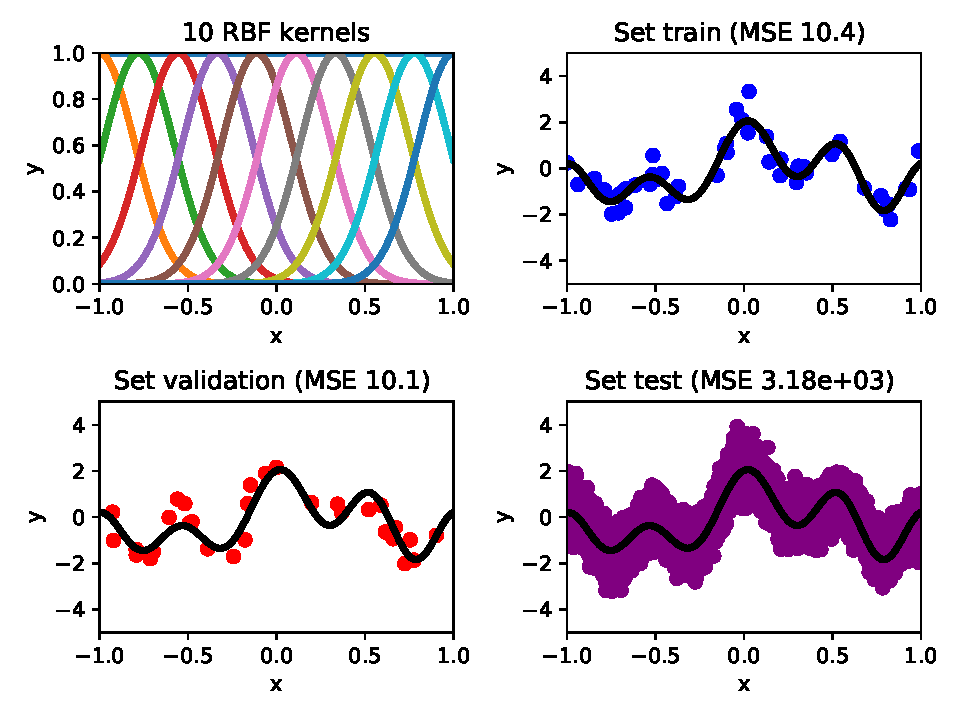
\includegraphics[width=\textwidth]{./Figures/linreg_rbf1_ncent10.pdf}
\caption{$l=10$}
\end{subfigure}
\begin{subfigure}{0.65\textwidth}
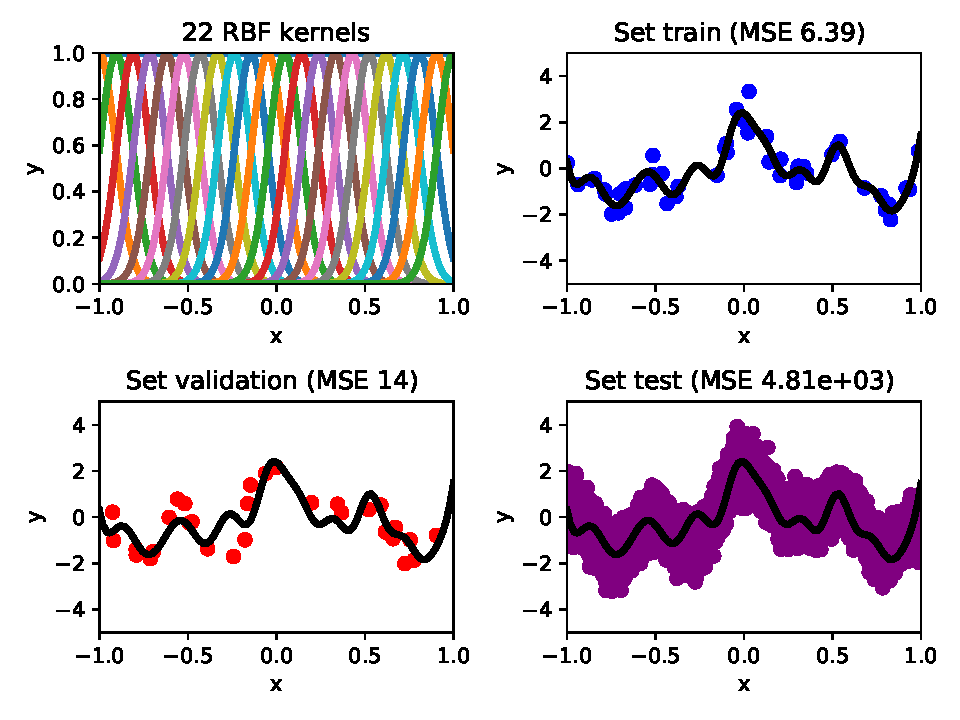
\includegraphics[width=\textwidth]{./Figures/linreg_rbf1_ncent22.pdf}
\caption{$l=22$}
\end{subfigure}
}
\caption{Results of Linear Regression for varying degree $l$.}
\label{linreg_rbf1}
\end{figure}

\begin{figure}[!ht]
\makebox[\textwidth]{
\begin{subfigure}{0.65\textwidth}
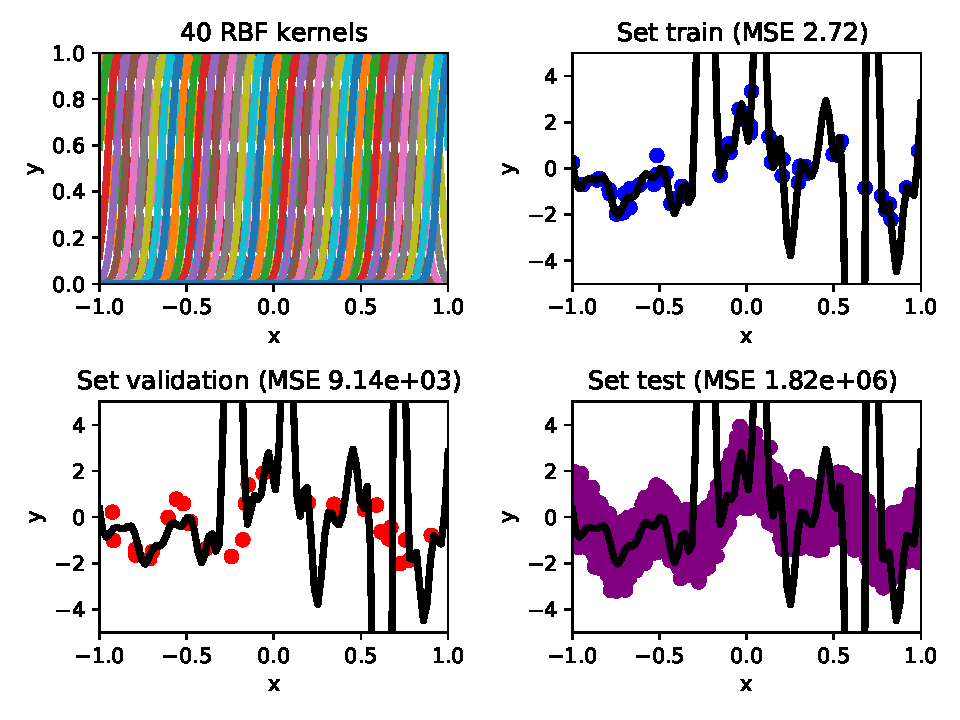
\includegraphics[width=\textwidth]{./Figures/linreg_rbf2_besttrain.pdf}
\caption{Training set, $l=40$}
\end{subfigure}
\begin{subfigure}{0.65\textwidth}
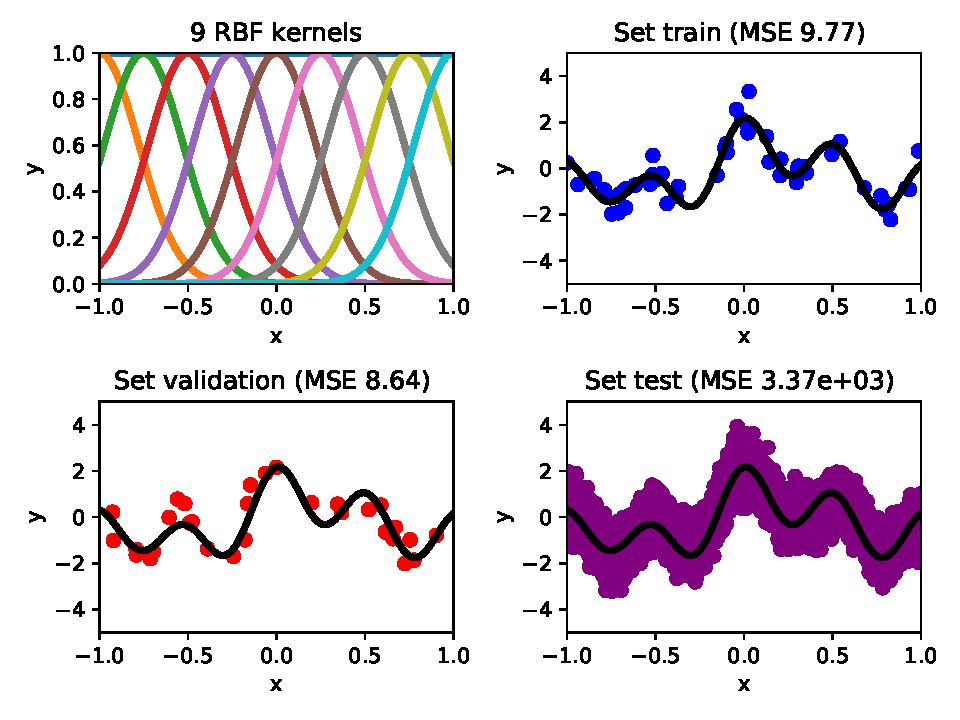
\includegraphics[width=\textwidth]{./Figures/linreg_rbf3_bestval.pdf}
\caption{Validation set, $l=9$}
\end{subfigure}
}
\caption{Results with lowest cost for training and validation set.}
\label{linreg_rbf23}
\end{figure}

\begin{figure}[!ht]
\centering
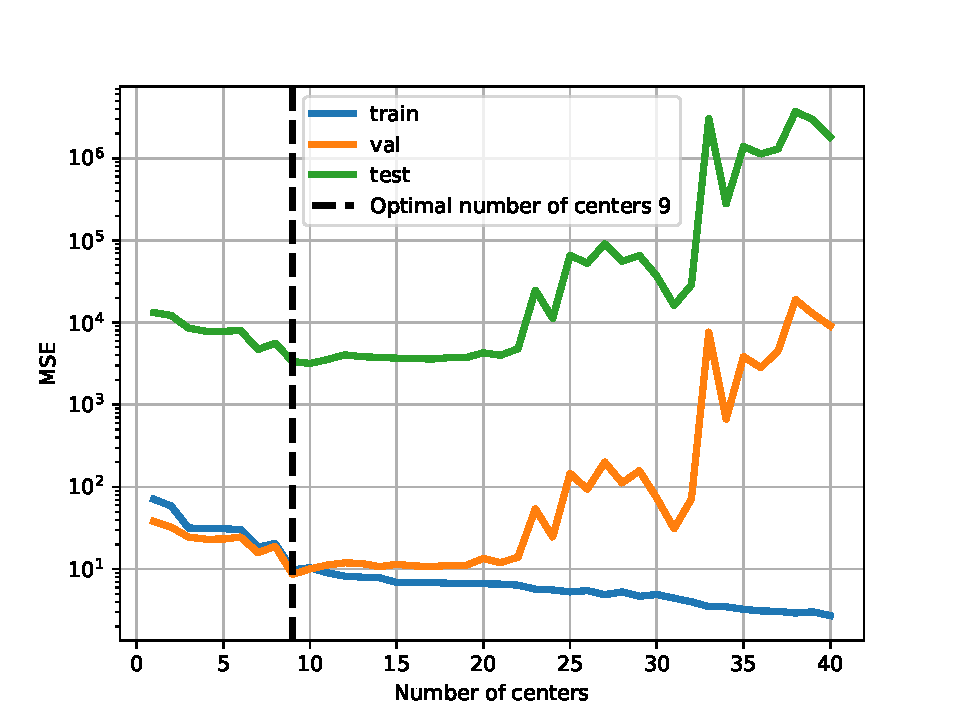
\includegraphics[width=0.8\textwidth]{./Figures/linreg_rbf4_errors.pdf}
\caption{Training, validation and testing costs as a function of the degree $l$.}
\label{linreg_rbf4}
\end{figure}

The results of the Linear Regression approach with radial basis functions are similar to the ones with polynomial functions: Increasing the degree/number of kernels $l$ leads to lower training cost (s. figure \ref{linreg_rbf4}) - minimised for $l=40$ (s. figure \ref{linreg_rbf23}) - but choosing $l$ too high results in overfitting (s. figure \ref{linreg_rbf1}). The cost function of the validation set is minimised for degree $l=9$ (s. figure \ref{linreg_rbf23}), leading to a low but not quite minimised testing cost. The actual testing cost minimum is found with degree $l=10$. Improving on the results of Linear Regression with polynomial basis functions it is about $20\%$ lower than the testing cost minimum with (higher) degree $n=13$ (s. figures \ref{linreg_rbf1} and \ref{linreg_poly23}). 


\clearpage

\section{Logistic Regression}

\subsection{Derivation of Gradient}

$$\begin{array}{rccl}
    J(\boldsymbol{\theta}) & = & - \frac{1}{m	} \displaystyle \sum_{i=1}^{m} \left(y^{(i)} \ \textrm{log}(h_{\boldsymbol{\theta}}(\boldsymbol{x}^{(i)})) + (1 - y^{(i)}) \ \textrm{log} (1 - h_{\boldsymbol{\theta}}(\boldsymbol{x}^{(i)}))\right) & \mid \frac{\partial}{\partial \boldsymbol{\theta}_j} \\\\
\end{array}$$
    
Derivation of the hypothesis function $ h_{\boldsymbol{\theta}}(\boldsymbol{x}) $:\

$$\begin{array}{rccl}  

&&\frac{\partial h_{\boldsymbol{\theta}}(\boldsymbol{x})}{\partial \theta_j} = \frac{\partial}{\partial \theta_j} \sigma(\theta_0 x_0 + \theta_1 x_1 + \dots + \theta_n x_n) = \sigma(\boldsymbol{x}^T\boldsymbol{\theta})\left(1-\sigma(\boldsymbol{x}^T\boldsymbol{\theta})\right)x_j = h_{\boldsymbol{\theta}}(\boldsymbol{x})\left(1-h_{\boldsymbol{\theta}}(\boldsymbol{x})\right)x_j&\\\\
\end{array}$$

Using the chain rule and the given hint for the derivation of the sigmoid function $\sigma$, we get:

$$\begin{array}{rccl}       
    \frac{J(\boldsymbol{\theta})}{\partial \theta_j} & = & -\frac{1}{m} \displaystyle \sum_{i=1}^{m}\left( y^{(i)} \frac{1}{h_{\boldsymbol{\theta}}(\boldsymbol{x}^{(i)})} h_{\boldsymbol{\theta}}(\boldsymbol{x}^{(i)}) \left(1 - h_{\boldsymbol{\theta}}(\boldsymbol{x}^{(i)})\right) \ x^{(i)}_j + \dots \right.  &  \\\\
    & & \left. \dots (1 - y^{(i)}) \frac{1}{1 - h_{\boldsymbol{\theta}}(\boldsymbol{x}^{(i)})} \left(-h_{\boldsymbol{\theta}}(\boldsymbol{x}^{(i)}) \ (1 - h_{\boldsymbol{\theta}}(\boldsymbol{x}^{(i)})) \ x^{(i)}_j\right) \right) \\\\
    \frac{J(\boldsymbol{\theta})}{\partial \theta_j} & = & -\frac{1}{m} \displaystyle \sum_{i=1}^{m}\left(y^{(i)} (1 - h_{\boldsymbol{\theta}}(\boldsymbol{x}^{(i)}) + h_{\boldsymbol{\theta}}(\boldsymbol{x}^{(i)})) - h_{\boldsymbol{\theta}}(\boldsymbol{x}^{(i)}) \right) x^{(i)}_j & \\\\
    \frac{J(\boldsymbol{\theta})}{\partial \theta_j} & = & \frac{1}{m} \displaystyle \sum_{i=1}^{m} \left(h_{\boldsymbol{\theta}}(\boldsymbol{x}^{(i)})-y^{(i)}\right) \ x^{(i)}_j
    
\end{array}$$

\newpage

\subsection{Logistic Regression training with gradient descent}

\begin{itemize}
\item What is the function \texttt{check\_gradient} doing?
\begin{itemize}
\item The cost $f_0$ and gradient $\boldsymbol{g}_0$ for a randomly chosen $\boldsymbol{x}_0$ are determined via the functions implemented in \texttt{logreg.py}. Then a random direction $\boldsymbol{dx}$ in which to check the gradient is generated and a scalar $df_g$ containing the sum of the gradient elements weighted by the elements of $\boldsymbol{dx}$ is computed via the dot product. For three predetermined deltas $d=10^{-2},10^{-4},10^{-6}$  the cost $f_1$ at $\boldsymbol{x}_0+d\cdot \boldsymbol{dx}$ is computed (again via the implemented function) and the gradient $df$ is determined as:

\begin{align*}
df = \frac{\Delta f}{\Delta x} = \frac{f_1-f_0}{d}
\end{align*}

Then the logarithm of the error $|df_g - df|$ is computed for each $d$ (the added constant $10^{-20}$ prevents the logarithm from becoming zero). If for decreasing $d$ the log-error always decreases by more than 1 or if all log-errors are smaller than -20 the gradient is well approximated and a confirmation message is printed. Otherwise an error is raised.
\end{itemize}

\begin{figure}[!ht]
\centering
\makebox[\textwidth]{
\begin{subfigure}{0.5\textwidth}
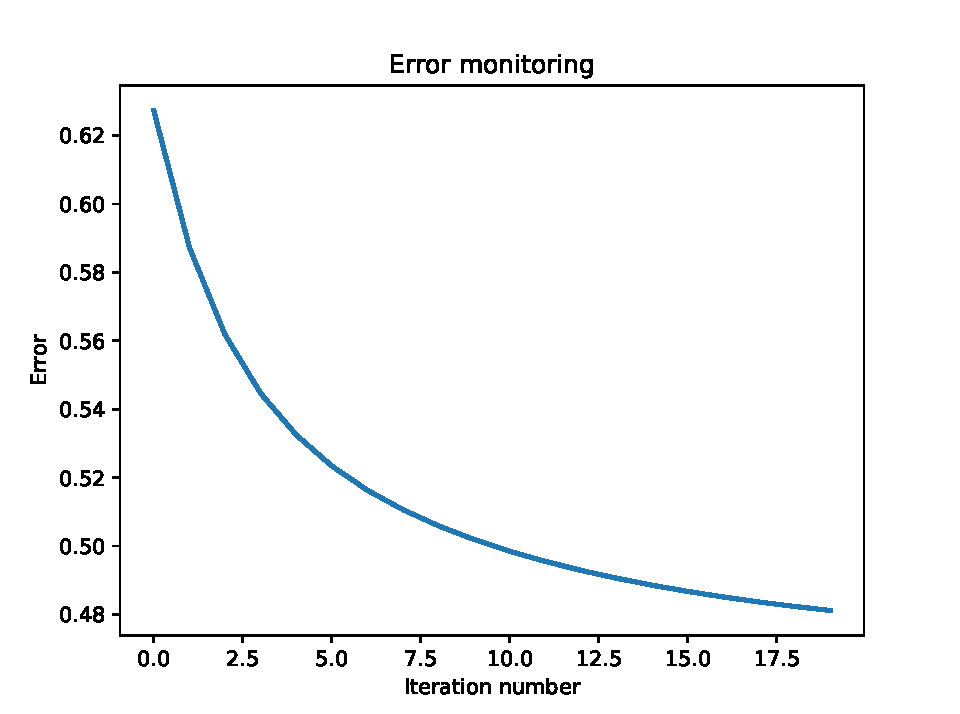
\includegraphics[width=\textwidth]{./Figures/logreg2_iter20_error.pdf}
\caption{Error, 20 iterations}
\end{subfigure}
\begin{subfigure}{0.5\textwidth}
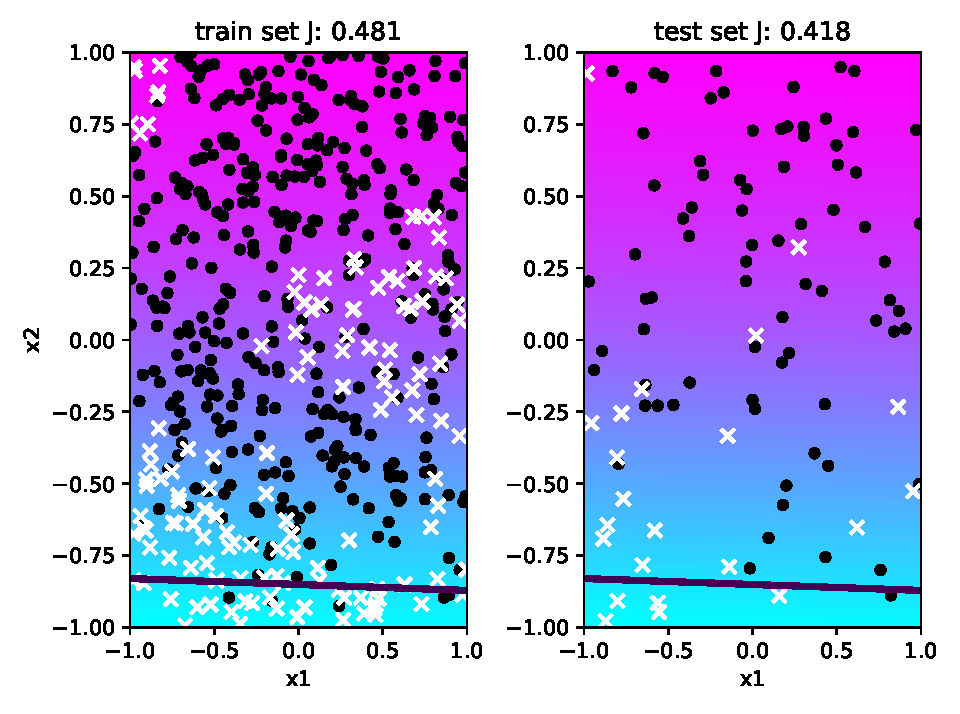
\includegraphics[width=\textwidth]{./Figures/logreg2_iter20_decbound.pdf}
\caption{Decision boundary, 20 iterations}
\end{subfigure}
}

\makebox[\textwidth]{
\begin{subfigure}{0.5\textwidth}
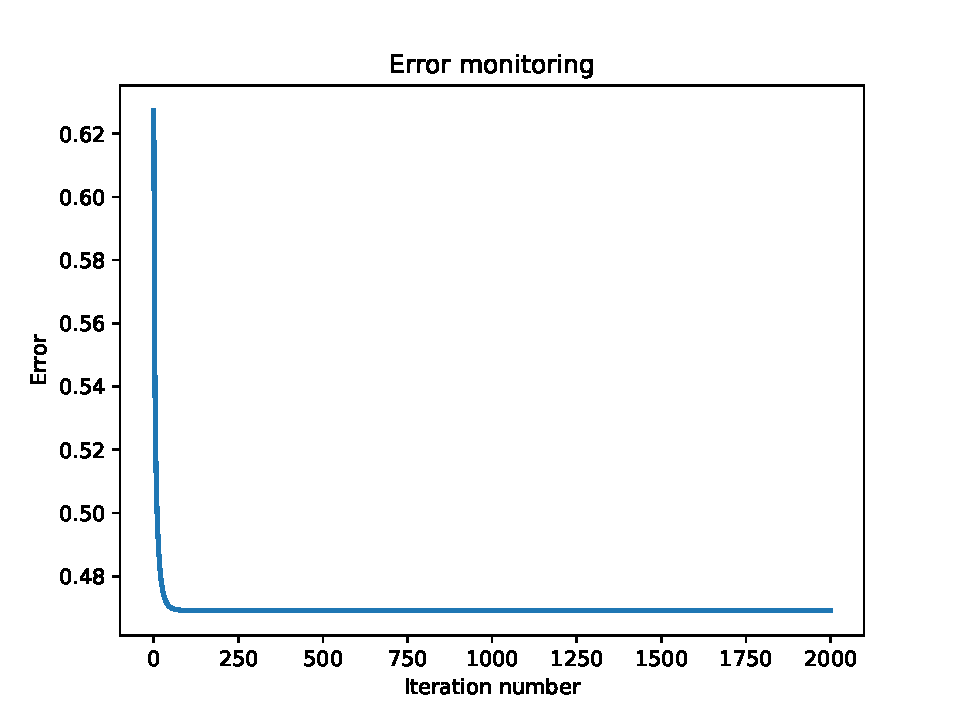
\includegraphics[width=\textwidth]{./Figures/logreg2_iter2000_error.pdf}
\caption{Error, 2000 iterations}
\end{subfigure}
\begin{subfigure}{0.5\textwidth}
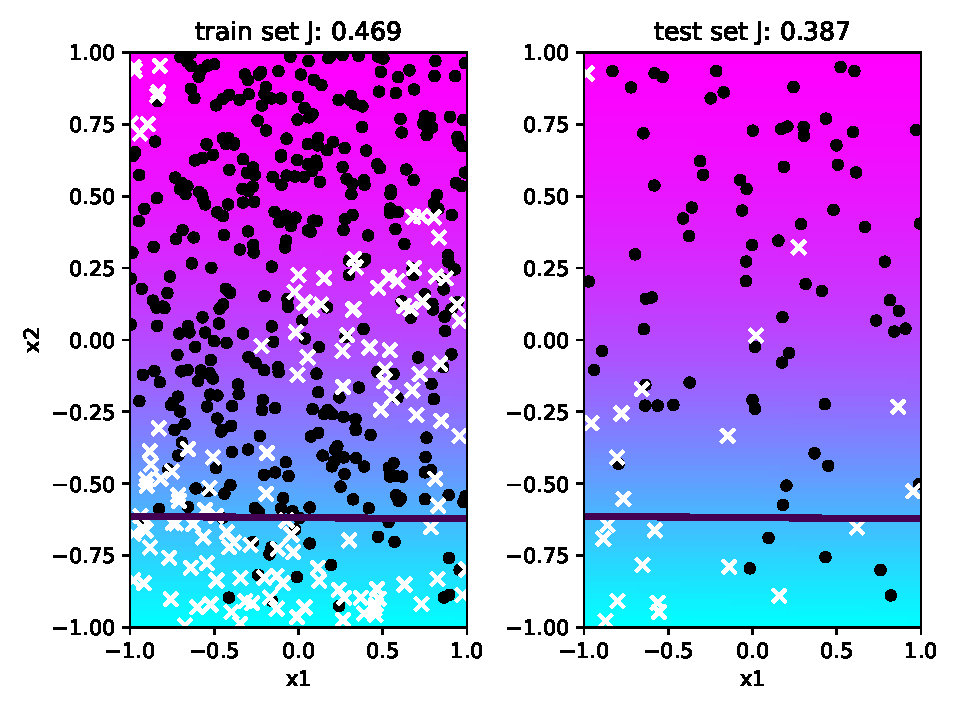
\includegraphics[width=\textwidth]{./Figures/logreg2_iter2000_decbound.pdf}
\caption{Decision boundary, 2000 iterations}
\end{subfigure}
}
\caption{GD errors and decision boundaries for varying number of iterations, degree $l=1$ and learning rate $\eta=1$.}
\label{logreg2}
\end{figure}

\item For degree $l=1$ and learning rate $\eta=1$ the GD was run for 20 and 2000 iterations (s. figure \ref{logreg2}). With only 20 iterations the GD algorithm stops before convergence leading to an inaccurate decision boundary and higher training and testing costs. Performing 2000 iterations one gets a more accurate decision boundary but the algorithm already converges after a fraction of the iterations, essentially wasting the majority of the computation time. A possible solution to prevent this would be the stopping criterion proposed at the end of this section.

\begin{figure}[!ht]
\centering
\makebox[\textwidth]{
\begin{subfigure}{0.5\textwidth}
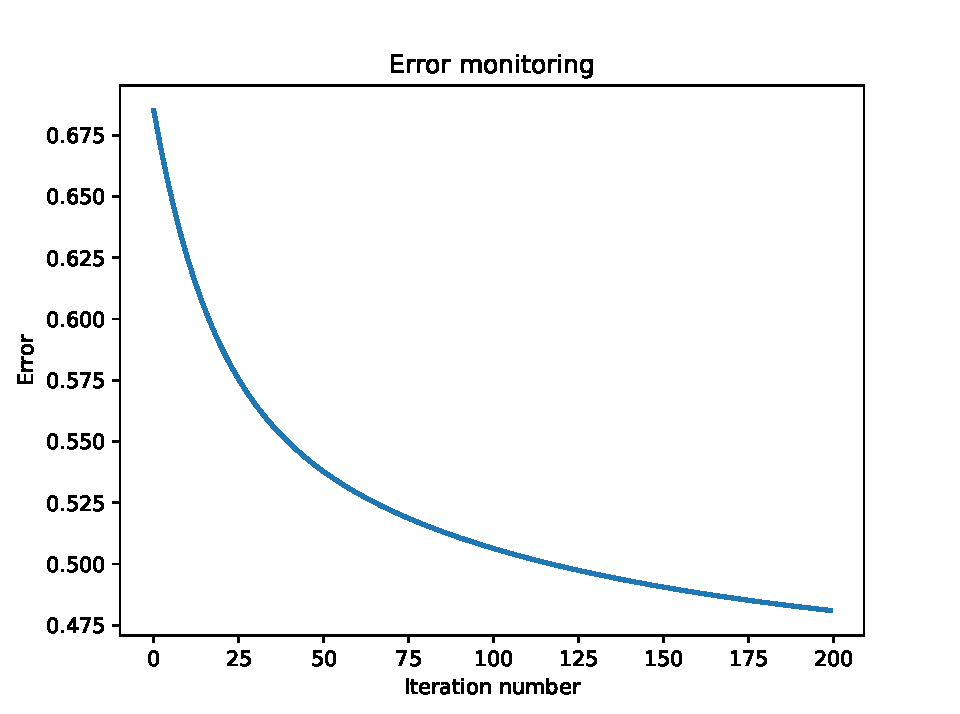
\includegraphics[width=\textwidth]{./Figures/logreg3_eta01_error.pdf}
\caption{Error, $\eta=0.1$}
\end{subfigure}
\begin{subfigure}{0.5\textwidth}
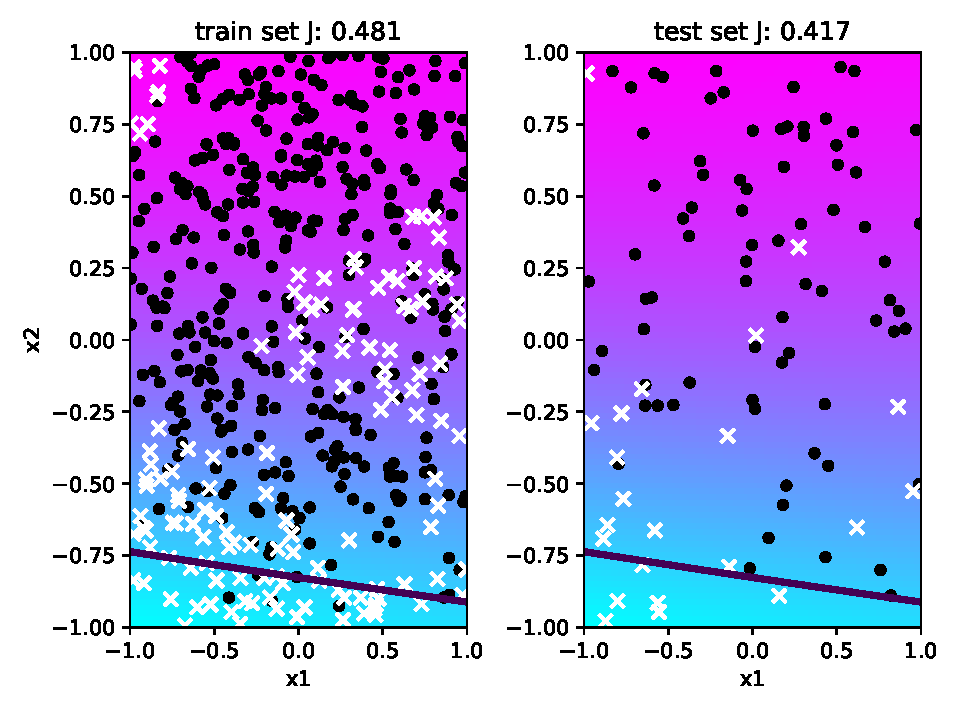
\includegraphics[width=\textwidth]{./Figures/logreg3_eta01_decbound.pdf}
\caption{Decision boundary, $\eta=0.1$}
\end{subfigure}
}

\makebox[\textwidth]{
\begin{subfigure}{0.5\textwidth}
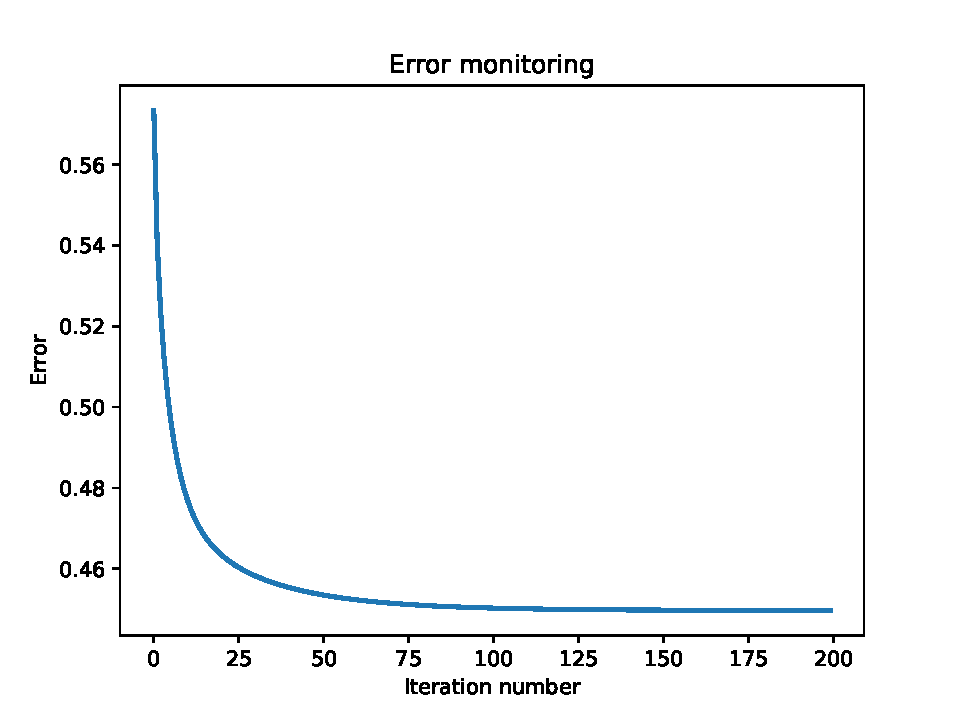
\includegraphics[width=\textwidth]{./Figures/logreg3_eta2_error.pdf}
\caption{Error, $\eta=2$}
\end{subfigure}
\begin{subfigure}{0.5\textwidth}
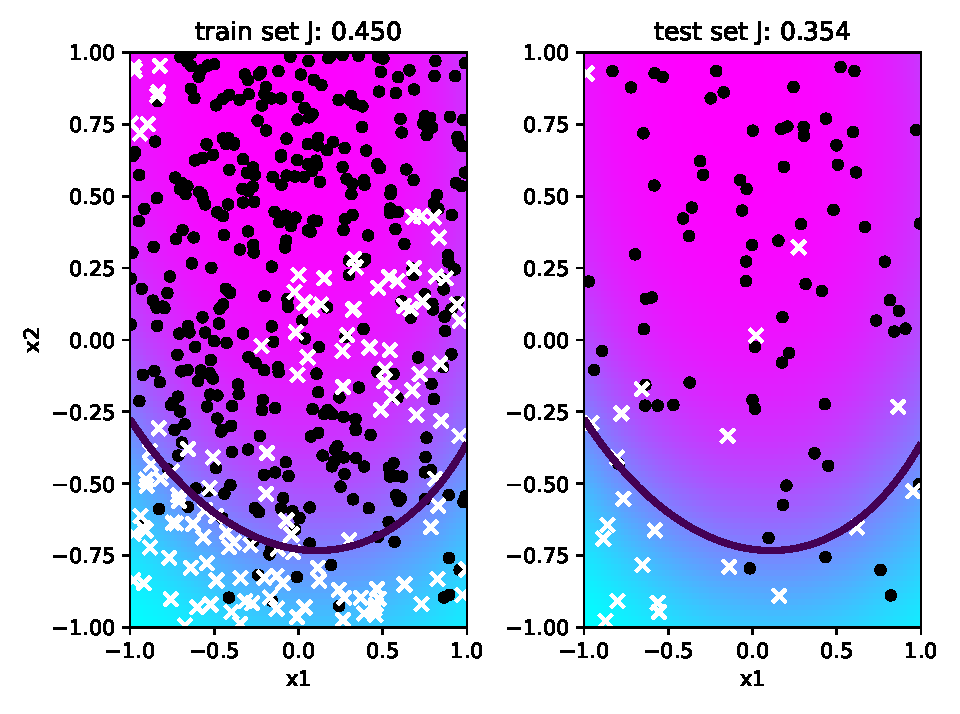
\includegraphics[width=\textwidth]{./Figures/logreg3_eta2_decbound.pdf}
\caption{Decision boundary, $\eta=2$}
\end{subfigure}
}

\makebox[\textwidth]{
\begin{subfigure}{0.5\textwidth}
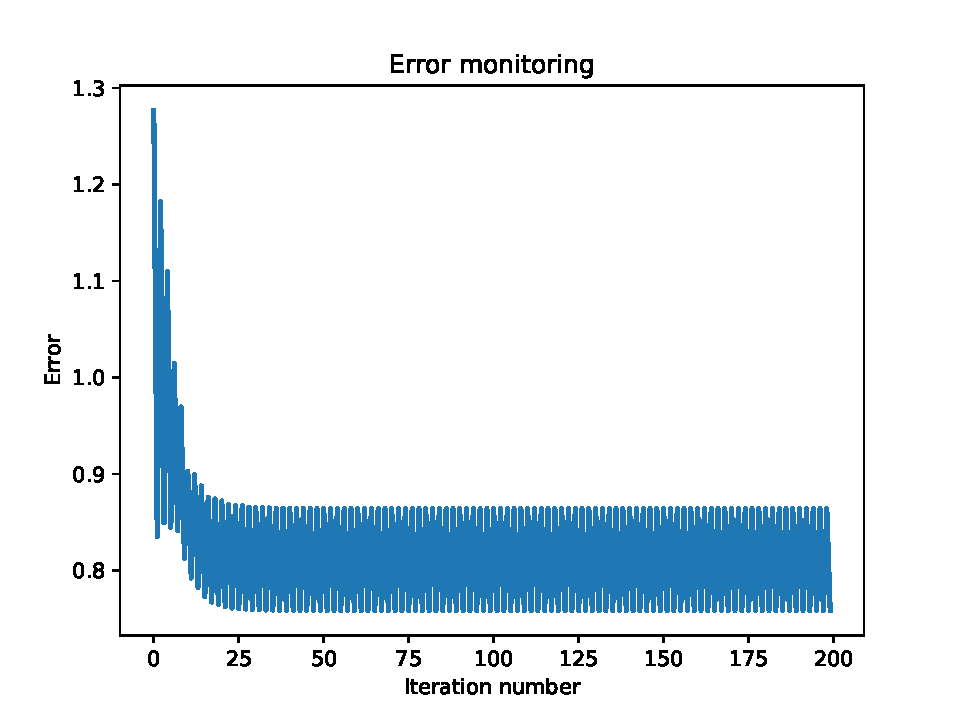
\includegraphics[width=\textwidth]{./Figures/logreg3_eta20_error.pdf}
\caption{Error, $\eta=20$}
\end{subfigure}
\begin{subfigure}{0.5\textwidth}
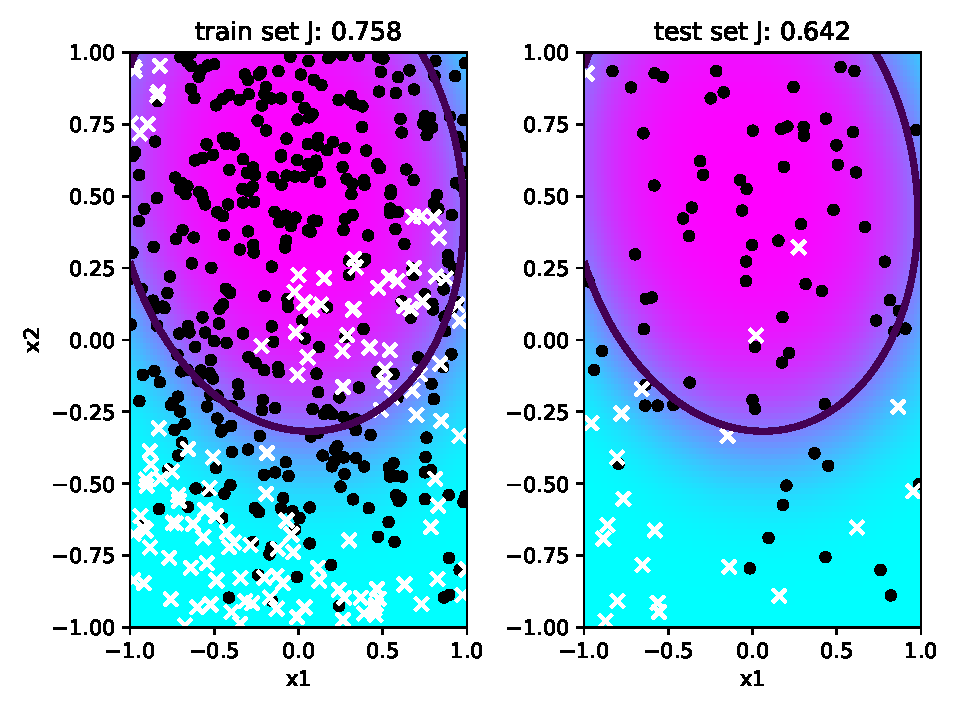
\includegraphics[width=\textwidth]{./Figures/logreg3_eta20_decbound.pdf}
\caption{Decision boundary, $\eta=20$}
\end{subfigure}
}
\caption{GD errors and decision boundaries for varying learning rate $\eta$, degree $l=2$ and 200 iterations.}
\label{logreg3}
\end{figure}

\item For degree $l=2$ the GD algorithm was run for 200 iterations with learning rates $\eta=0.1,2,20$ (s. figure \ref{logreg3}). The learning rate $\eta = 0.1$ is too small, preventing the algorithm from converging in time. The result is an inaccurate decision boundary and higher training and testing costs. $\eta = 2$ works well with the other set parameters. The GD algorithm converges, the decision boundary works is quite accurate considering the low degree used and the training and testing costs are the lowest of the three results. The last learning rate  $\eta=20$ on the other hand is much too large. Rather than reaching the location of the minimum the algorithm overshoots repeatedly, preventing convergence and causing the algorithm to oscillate. Of course the resulting decision boundary is basically useless and the training and testing costs are very high.

\begin{figure}[!ht]
\vspace*{-53.6pt}
\centering
\makebox[\textwidth]{
\begin{subfigure}{0.5\textwidth}
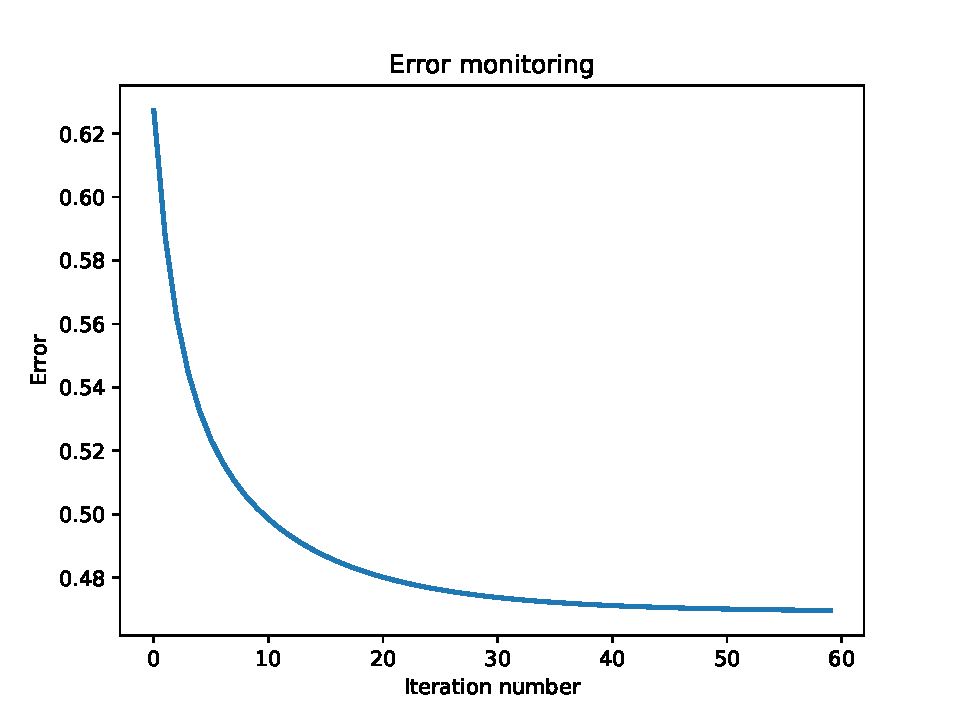
\includegraphics[width=\textwidth]{./Figures/logreg4_deg1_opt_error.pdf}
\caption{Error, $l=1$, $\eta=1$, 60 iterations}
\end{subfigure}
\begin{subfigure}{0.5\textwidth}
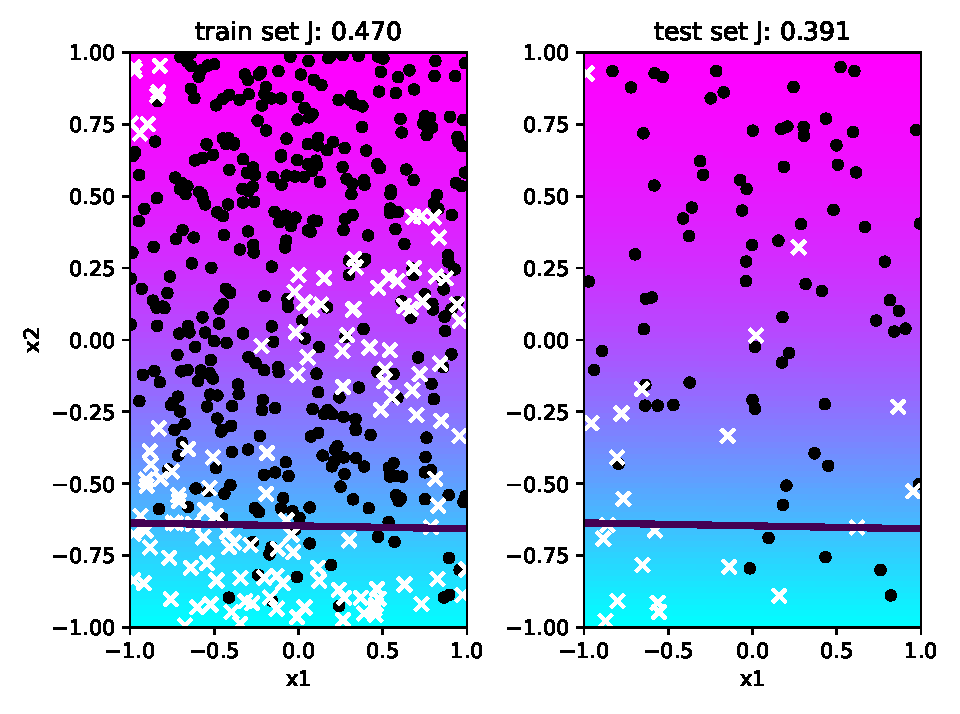
\includegraphics[width=\textwidth]{./Figures/logreg4_deg1_opt_decbound.pdf}
\caption{Decision boundary, $l=1$, $\eta=1$, 60 iterations}
\end{subfigure}
}

\makebox[\textwidth]{
\begin{subfigure}{0.5\textwidth}
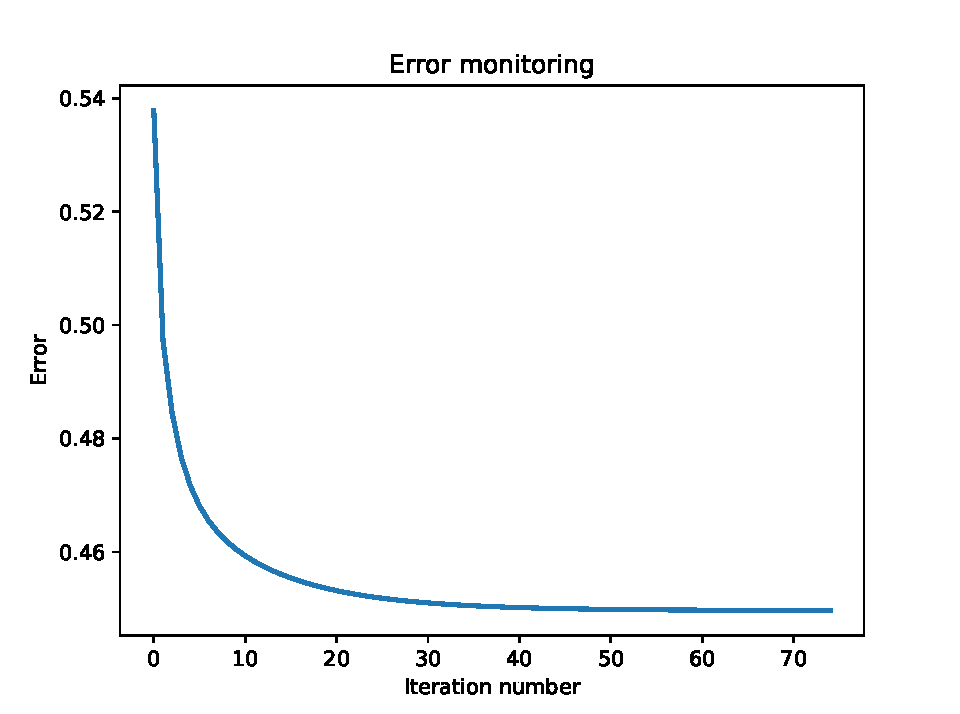
\includegraphics[width=\textwidth]{./Figures/logreg4_deg2_opt_error.pdf}
\caption{Error, $l=2$, $\eta=5$, 75 iterations}
\end{subfigure}
\begin{subfigure}{0.5\textwidth}
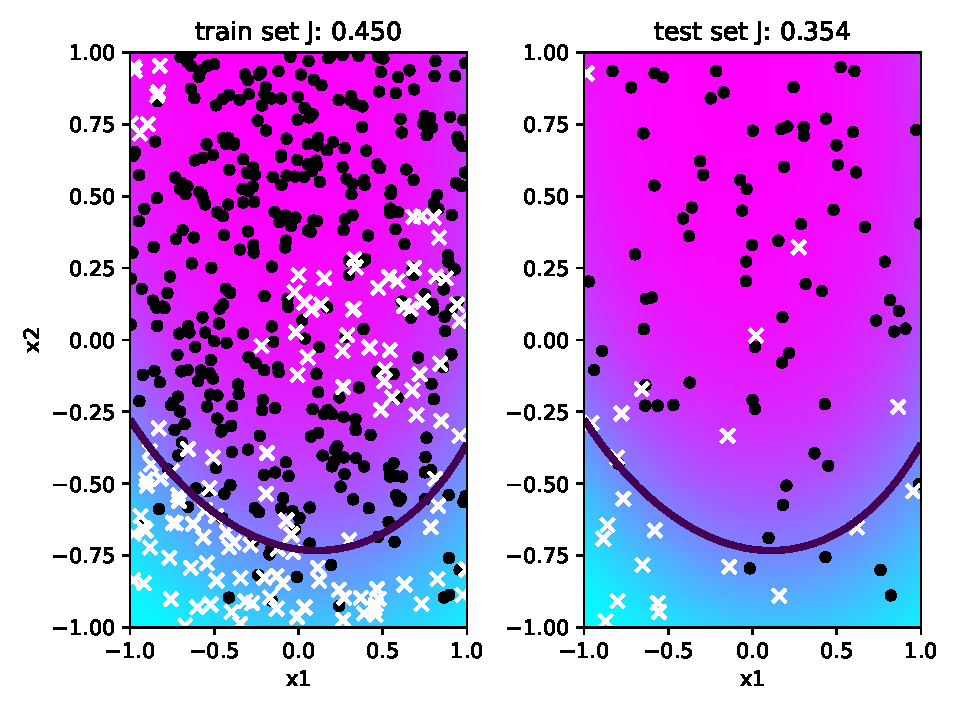
\includegraphics[width=\textwidth]{./Figures/logreg4_deg2_opt_decbound.pdf}
\caption{Decision boundary, $l=2$, $\eta=5$, 75 iterations}
\end{subfigure}
}

\makebox[\textwidth]{
\begin{subfigure}{0.5\textwidth}
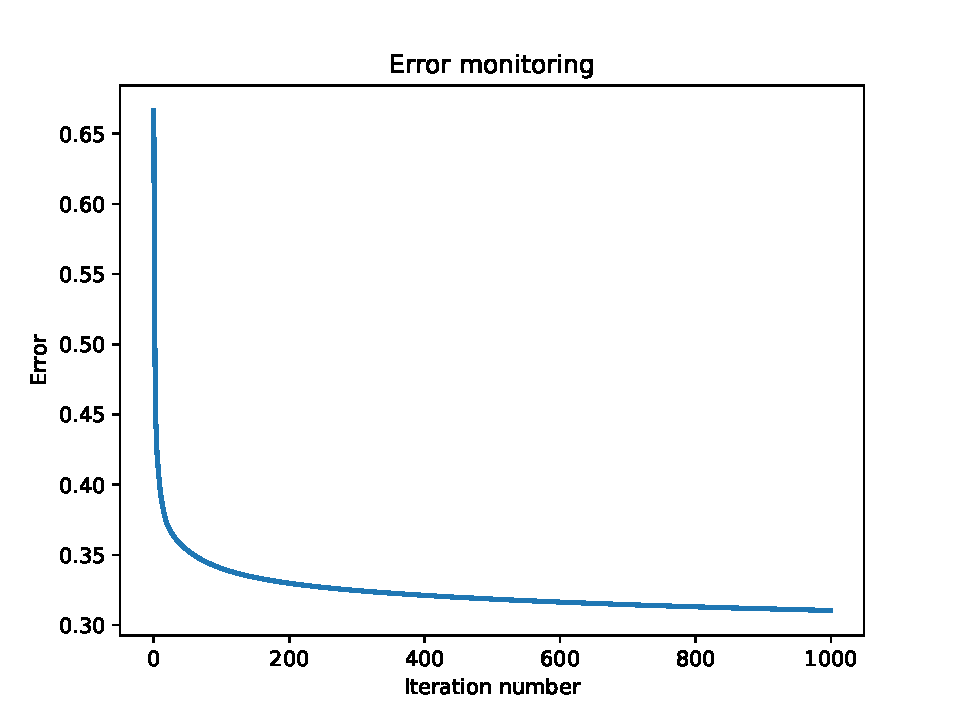
\includegraphics[width=\textwidth]{./Figures/logreg4_deg7_opt_error.pdf}
\caption{Error, $l=7$, $\eta=10$, 1000 iterations}
\end{subfigure}
\begin{subfigure}{0.5\textwidth}
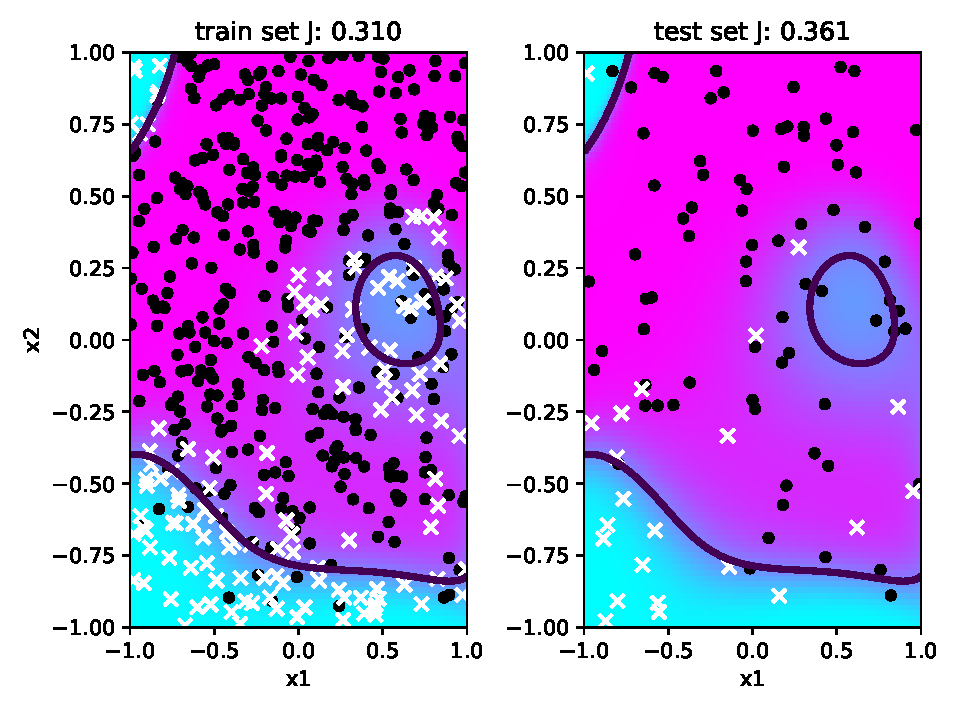
\includegraphics[width=\textwidth]{./Figures/logreg4_deg7_opt_decbound.pdf}
\caption{Decision boundary, $l=7$, $\eta=10$, 1000 iterations}
\end{subfigure}
}

\makebox[\textwidth]{
\begin{subfigure}{0.5\textwidth}
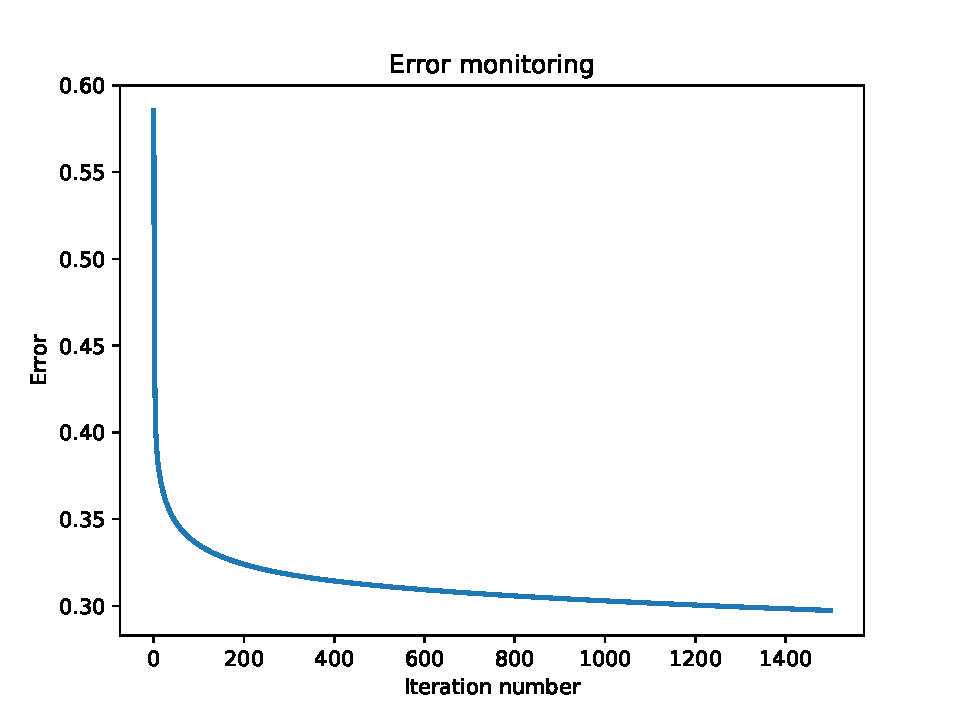
\includegraphics[width=\textwidth]{./Figures/logreg4_deg20_opt_error.pdf}
\caption{Error, $l=20$, $\eta=8$, 1500 iterations}
\end{subfigure}
\begin{subfigure}{0.5\textwidth}
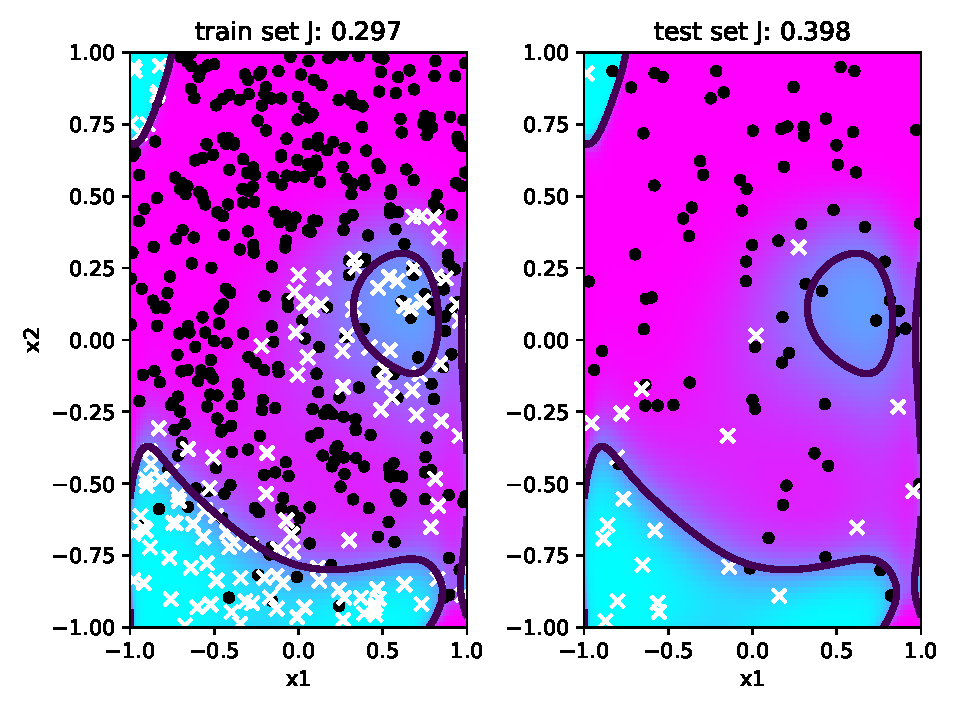
\includegraphics[width=\textwidth]{./Figures/logreg4_deg20_opt_decbound.pdf}
\caption{Decision boundary, $l=20$, $\eta=8$, 1500 iterations}
\end{subfigure}
}
\caption{GD errors and decision boundaries for degrees $l=1,2,7,20$ and chosen parameter values.}
\label{logreg4_fig}
\end{figure}

\item For degrees $l=1,2,7,20$ reasonably good pairs of values for the number of iterations and learning rate have been identified (s. figure \ref{logreg4_fig} and table \ref{logreg4_tab}). Especially with higher degrees it has turned out to be quite difficult to find the right balance between keeping the computational time at acceptable levels and finding good learning rates, because even after the initial steep descent the error continues to slowly decrease. Of all tested degrees $l=7$ seems to fit the data best although the testing cost is slightly lower with $l=2$. The lowest training cost is obtained by using $l=20$ but this results in overfitting.

\begin{table}[!ht]
\centering
\begin{tabular}{|c||c|c||c|c|}
\hline
degree $l$ & learning rate $\eta$ & iterations & training cost & testing cost \\ \hline \hline
1          & 1                    & 60         & 0.470         & 0.391        \\ \hline
2          & 5                    & 75         & 0.450         & 0.354        \\ \hline
7          & 10                   & 1000       & 0.310         & 0.361        \\ \hline
20         & 8                    & 1500       & 0.297         & 0.398        \\ \hline
\end{tabular}
\caption{Chosen values for learning rate $\eta$ and number of iterations and obtained training and testing costs for degrees $l=1,2,7,20$.}
\label{logreg4_tab}
\end{table}

\item What could a possible stopping criterion look like?

\begin{itemize}
\item In the GD update equation $\boldsymbol{\theta} = \boldsymbol{\theta} - \eta \nabla_{\boldsymbol{\theta}} J(\boldsymbol{\theta})$ the elements of the gradient vector contain the updates for each dimension of $\boldsymbol{\theta}$. If an element of the gradient is very small the solution will only change very little in that dimension. So on each iteration of the GD before updating $\boldsymbol{\theta}$ one could compare the elements of the gradient to a threshold. If all elements are smaller than the threshold the location of the minimum of the cost function is reasonably well approximated and the update loop can be aborted.
\end{itemize}
\end{itemize}

\end{document}